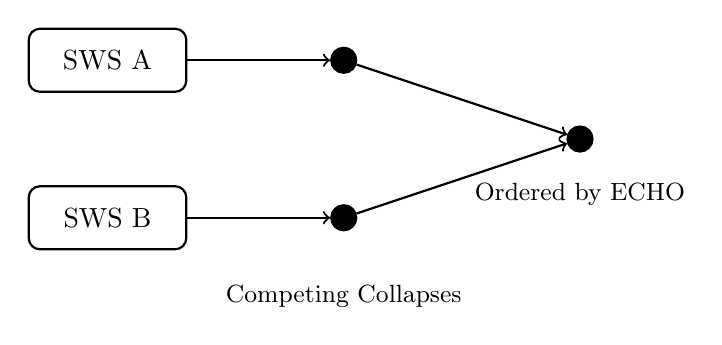
\begin{tikzpicture}[
    sws/.style={rectangle, draw=black, thick, rounded corners, minimum width=2cm, minimum height=0.8cm, align=center},
    collapse/.style={circle, draw=black, fill=black, minimum size=6pt},
    echo/.style={->, thick},
]

\node[sws] (A) at (0,0) {SWS A};
\node[sws] (B) at (0,-2) {SWS B};

\node[collapse] (a1) at (3,0) {};
\node[collapse] (b1) at (3,-2) {};

\node[collapse] (next) at (6,-1) {};

\draw[echo] (A) -- (a1);
\draw[echo] (B) -- (b1);

\draw[echo] (a1) -- (next);
\draw[echo] (b1) -- (next);

\node at (3,-3) {\small Competing Collapses};
\node at (6,-1.7) {\small Ordered by ECHO};

\end{tikzpicture}